\begin{spacing}{1}
    \chapter*{Abstract}
\end{spacing}
\subsubsection{Task}
The task was to program a new test program for the train drives of the ÖBB Technical Service Linz. Because this task
turned out to be too extensive for this work, it was agreed upon that an evaluation program for the errors of the currently
used program was to be made. This program should filter and display errors according to various criteria, which should 
increase error detection in productive operation.
\subsubsection{Implementation}
The implementation was done in Csharp and Angular as we already had experience with these programming languages. 
We get the data which is used in this project from QTX-Files that we recieved from the ÖBB-TS Linz.
This data is then evaluated in the backend and displayed in the frontend.
\subsubsection{Result}
An application with the basic functionalities was created. These functionalities can be expanded in the future by, 
for example, more criteria or a connection to the program which is used in productive operation.
\begin{center}
  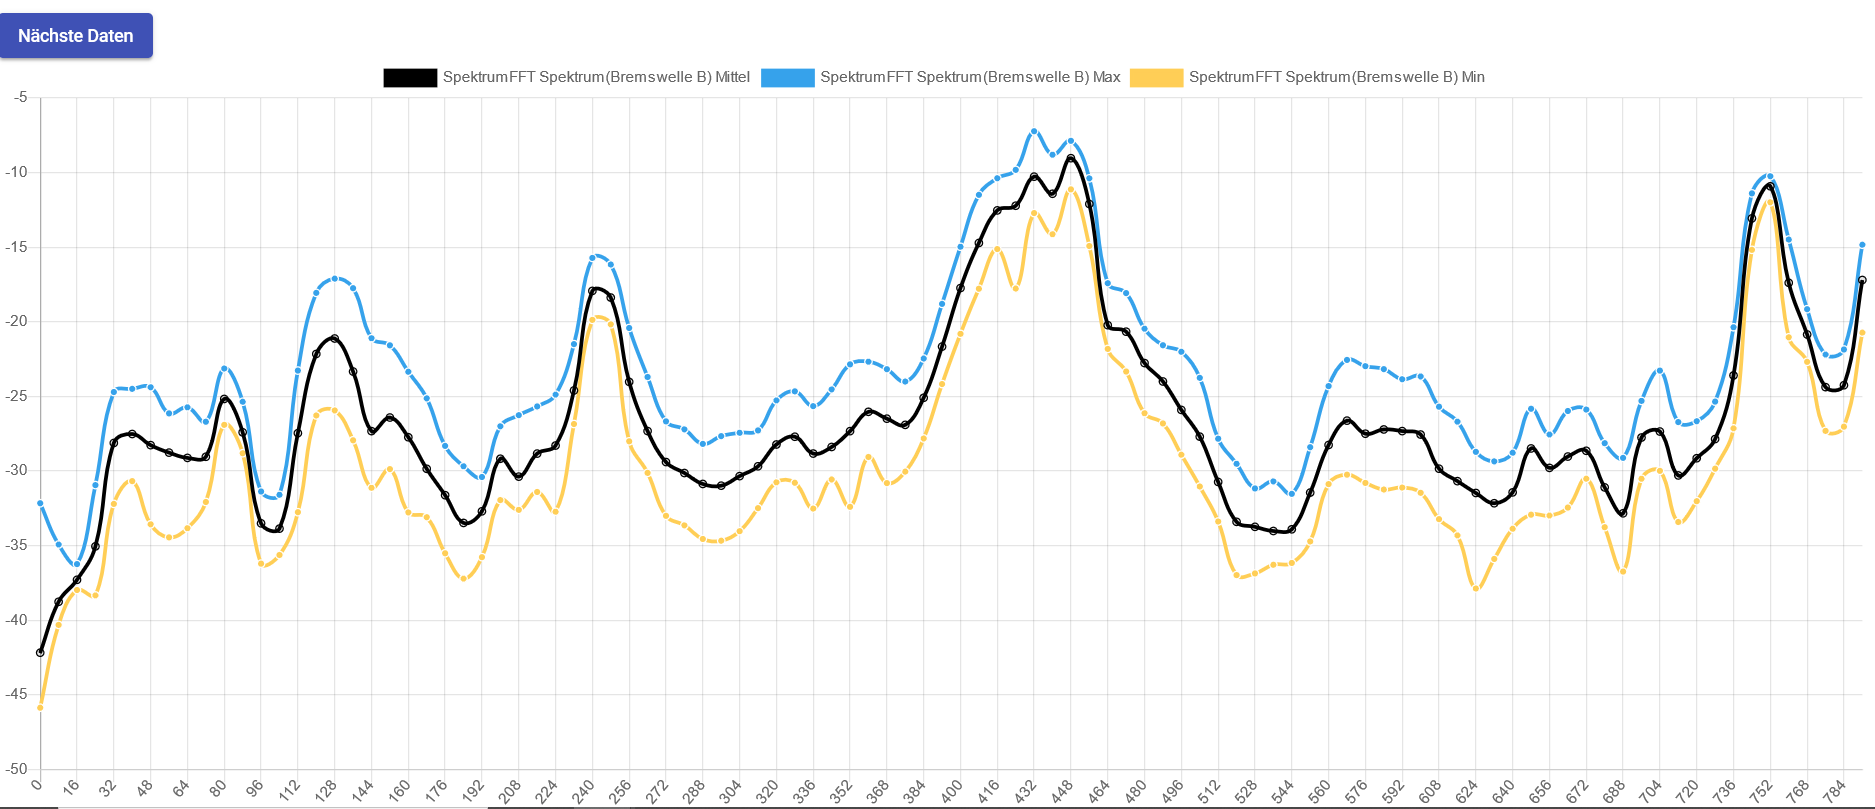
\includegraphics[width=0.8\textwidth]{pics/graphwok.PNG}
\end{center}
\newpage
\begin{spacing}{1}
    \chapter*{Zusammenfassung}
\end{spacing}
\subsubsection{Aufgabenstellung}
Aufgabe war es, ein neues Prüfprogramm für die Zugantriebe des ÖBB Technischen Service Linz zu programmieren. Da sich diese Aufgabe 
für diese Arbeit als zu umfangreich herausgestellt hat, wurde sich darauf geeinigt, ein Auswertungsprogramm für die Fehler des derzeit
eingesetzten Prüfprogramms zu programmieren. Dieses Programm soll die Fehler nach verschiedenen Kriterien filtern und darstellen
können, was die Fehlererkennung im Produktivbetrieb erhöhen soll.
\subsubsection{Realisierung}
Die Implementierung wurde in Csharp und Angular durchgeführt, da wir bereits Erfahrung mit diesen Programmiersprachen hatten. Die Daten, 
welche in diesem Projekt benutzt werden, werden aus QTX-Dateien, die wir von dem ÖBB-TS Linz zur Verfügung gestellt bekommen haben,
eingelesen und danach im Backend ausgewertet. Im Frontend werden die ausgewerteten Daten angezeigt.
\subsubsection{Ergebnis}
Es wurde eine Applikation erstellt, die grundsätzlich die vereinbarten Funktionalitäten enthält. Diese Funktionalitäten können in
Zukunft durch beispielsweise mehr Kriterien oder einer Anbindung an das im Produktivbetrieb benutzte Prüfprogramm erweitert werden.
\begin{center}
  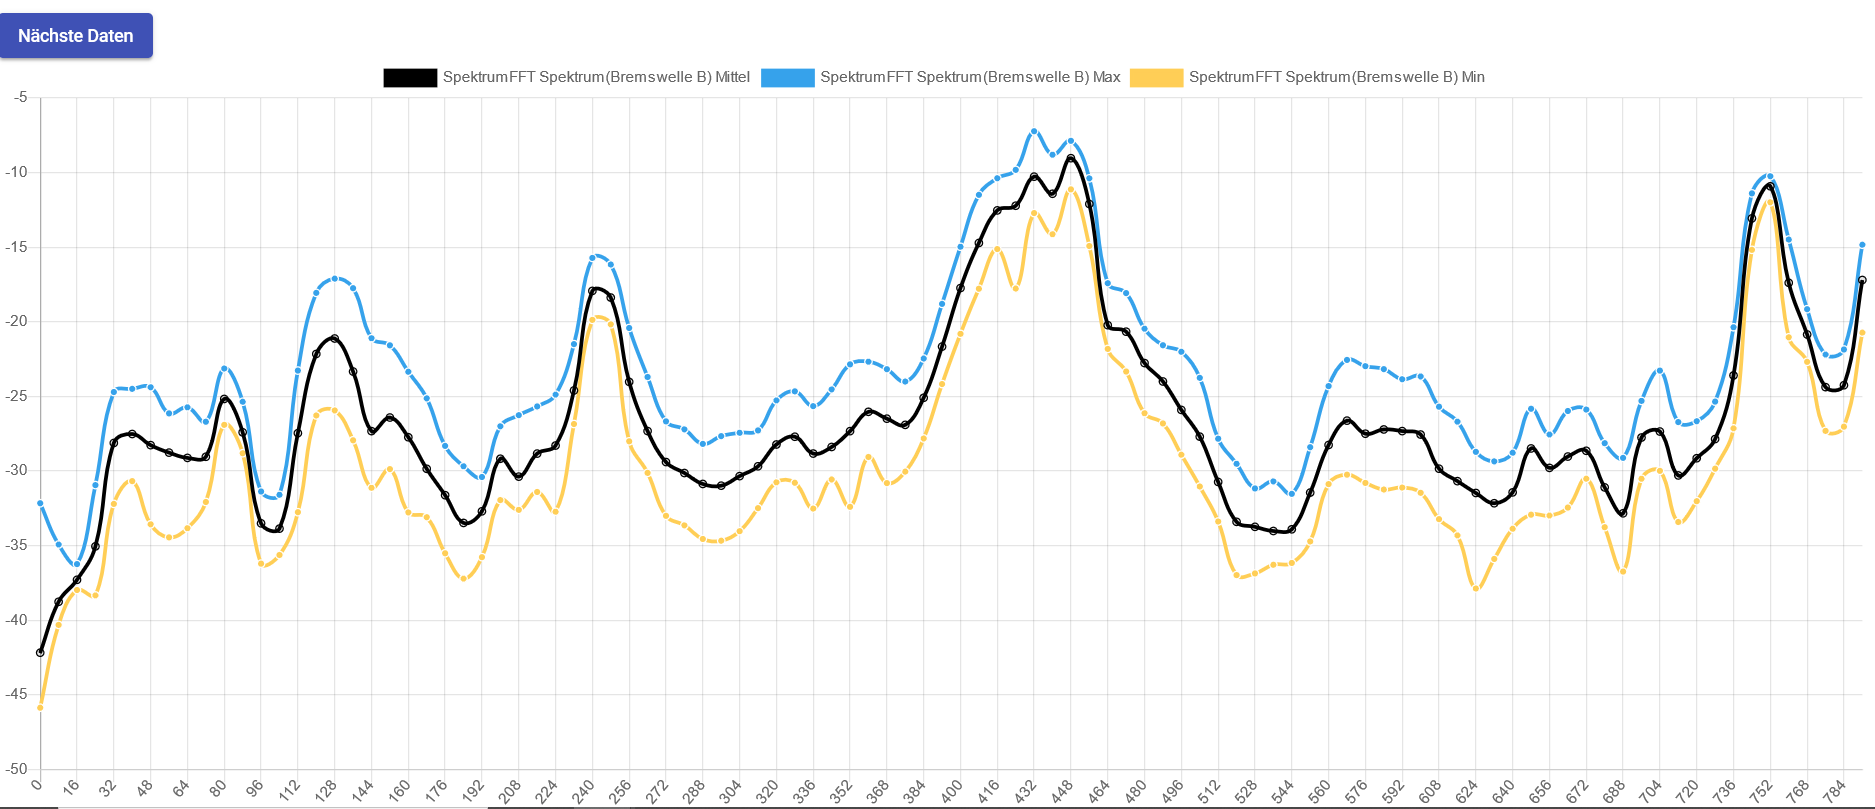
\includegraphics[width=0.8\textwidth]{pics/graphwok.PNG}
\end{center}
